\section{Analyse}
%Liste de questions et graphiques dans le protocole
\subsection{Courbes de base présentant le comportement de la turbine}
		\begin{figure}[H]
    			\centering
			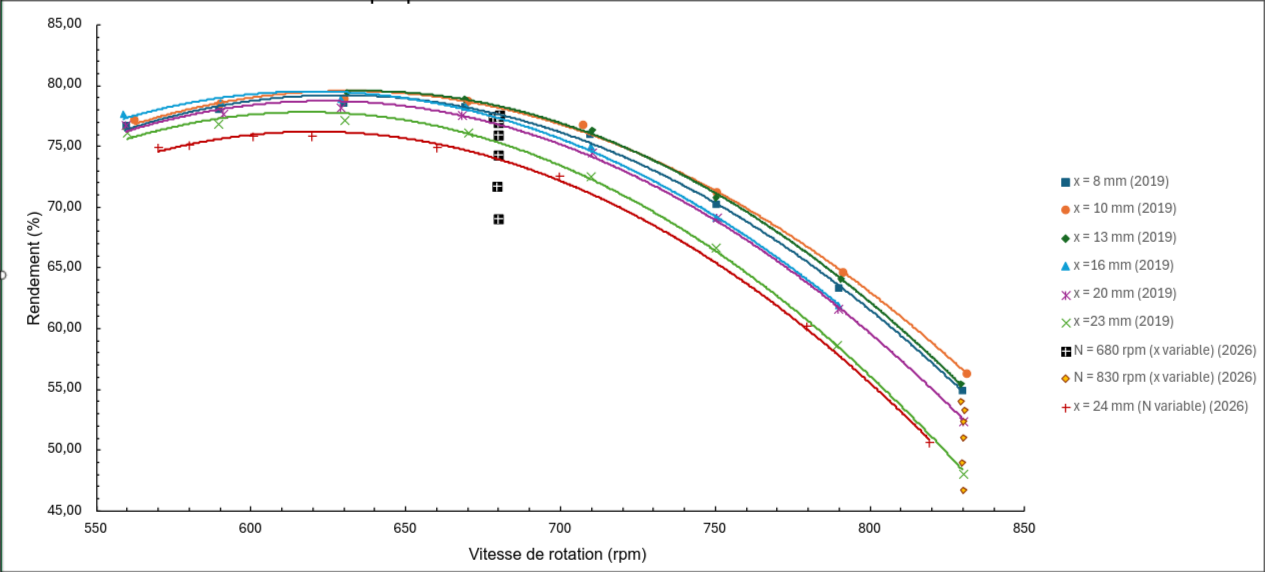
\includegraphics[width=\linewidth]{images/graphs/01_Rendement_rotation.png}
			\caption{Courbes de rendement en fonction de la vitesse de rotation}
    			\label{fig:Graph11}
		\end{figure}
 Malgré les différentes positions du pointeau, la vitesse de rotation à laquelle on obtient le meilleur rendement reste à peu près la même, soit à environ 630 rpm pour les courbes de 2019 et à environ 620 rpm pour la courbe expérimentale de 2026 (en rouge).
 Il est à noter que selon la figure 4.13 des notes de cours (source), le maximum se déplace légèrement selon l’ouverture du pointeau.
 Ainsi, puisque $C_1$ varie un peu avec le débit puisque pour la courbe expérimentale de 2026 avec le pointeau à x = 24 mm, cela correspond à une plus petite ouverture que les courbes de 2019 à x = 8 à 16 mm.
 Cela explique le léger décalage attendu. 
 Cependant, la courbe de 2019 à x = 23 mm est à une ouverture comparable et également à environ 630 rpm l’écart observé pourrait donc aussi venir d’autres facteurs, comme l’usure des paliers de la turbine, le vieillissement de la turbine, les capteurs, le pointeau et les PID qui n’ont pas été recalibré depuis quelques années, les pertes dans l’injecteur est la tuyauterie qui ont changé avec les années, les fuites du réservoirs au fil des années et la température de l’eau légèrement différente de celle de 2019.
 Tout cela peut changer soit le débit, les pertes ou les mesures et ainsi, le rendement entre les données de 2019 et celle de 2026.
 
 Au niveau de la théorique, le rendement maximal est obtenu lorsque $U = \frac{C_1}{2}$. Avec $C_1 \approx$ 26,09 m/s, on trouve U $\approx$ 13,05 m/s, d’où $\omega$ = $\frac{U*2}{D}$ $\approx$ 68,5 rad/s avec D = 0,381 m, ce qui donne N $\approx$ 654 rpm.
 Cette valeur est très proche de celle observée sur le graphique (620 à 630 rpm).
 L’écart d’environ 4\% s’explique, comme l’indiquent les notes de cours (figure 4.10, source) que le rapport de vitesse $\frac{U}{C_1}$ au maximum du rendement réel est plus petit que celui du rendement théorique (0,5), à cause des pertes dans l’injecteur et la tuyauterie.
 Dans notre cas, le maximum se situe à environ 620 rpm ou 630 rpm, soit $\frac{U}{C_1}$ $\approx$ 0,47 ou 0,48, au lieu de 0,5 (654 rpm). 

 Pour la forme des courbes, le polynôme d’ordre 2 utilisé pour les courbes de tendance est justifié, puisque le rendement théorique $\eta_{th} = (\frac{2*U}{C_1})(1 - \frac{U}{C_1})(1-kcos\alpha)$ est une parabole en fonction de N. Cela permet de bien suivre les données. Au-delà de $U = \frac{C_1}{2}$, le rendement diminue de plus en plus rapidement, car la vitesse relative du jet sur les augets ($C_1 - U$) devient de plus en plus petite. Ainsi, il y a moins d’énergie qui est transférée à la roue. Cette parabole est aussi plate près de $U = \frac{C_1}{2}$, ce qui explique que les vitesses d’opération soient relativement larges ce qui est en accord avec la théorie. De plus, il est intéressant de noter que le rendement reste au-dessus de 65\% jusqu’à environ 750 rpm et qu’il est également au-dessus de 70\% à 570 rpm confirmant la large bande d’utilisation des turbines Pelton. 

 Pour l’effet de l’ouverture du pointeau, il est visible sur les données de 2019 puisque de x = 8 à x = 16 mm, le rendement maximal est d’environ 79\% pour toutes les ouvertures.
 Il diminue lorsque la charge est faible (pointeau plus avancé), comme le montre la figure 4.14 des notes de cours (sources).
 À faible charge, le rendement de l’injecteur est plus bas.
 Ainsi, le jet est plus mince et les pertes à l’écoulement sont relativement plus grandes.
 Les deux courbes expérimentales à vitesse constante confirment cette tendance puisqu’ à 680 rpm, le rendement passe de 77,5\%.
 À x = 10 mm, il passe à 69,1\%. À partir de x = 30 mm, le débit chute de 23,0 à 8,8 kg/s.
 À 830 rpm, le rendement est beaucoup plus bas (54,0\% à x = 10 mm et 40,8\% à x = 30 mm), car cette vitesse est bien supérieure à la vitesse optimale ($\frac{C_1}{U}$ = 1,58 au lieu de 2, donc $U > \frac{C_1}{2}$).

		\begin{figure}[H]
    			\centering
			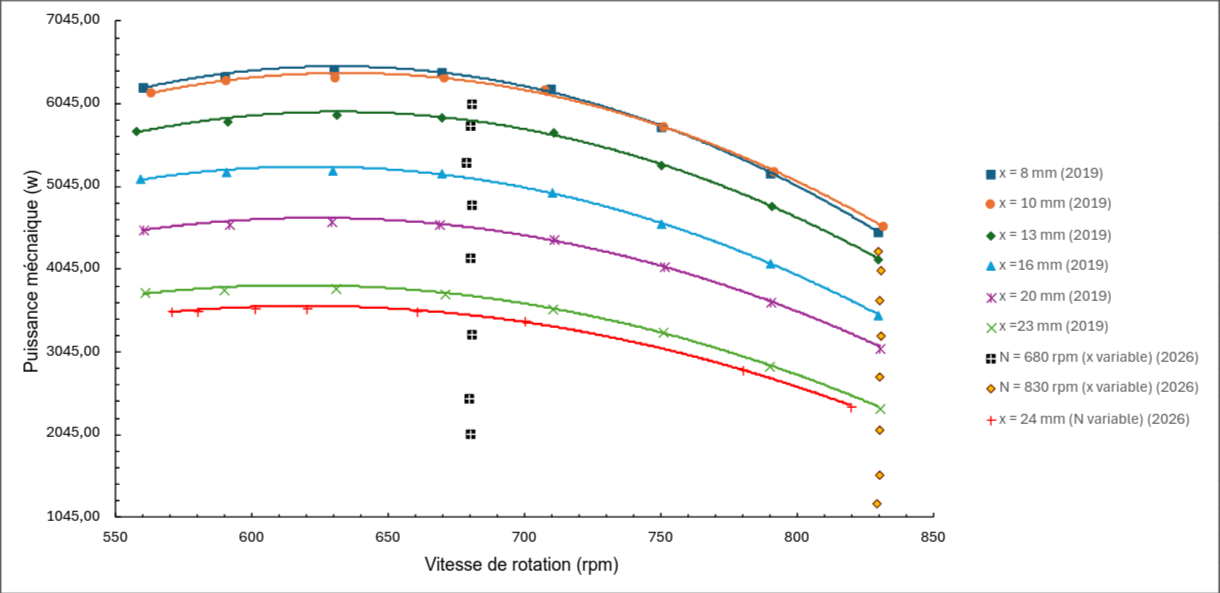
\includegraphics[width=\linewidth]{images/graphs/02_puissance_rotation.png}
			\caption{Courbes de puissance mécanique en fonction de la vitesse de rotation}
    			\label{fig:Graph12}
		\end{figure}

\subsection{Étude du transfert d'énergie entre le jet et la roue}
		\begin{figure}[H]
    			\centering
			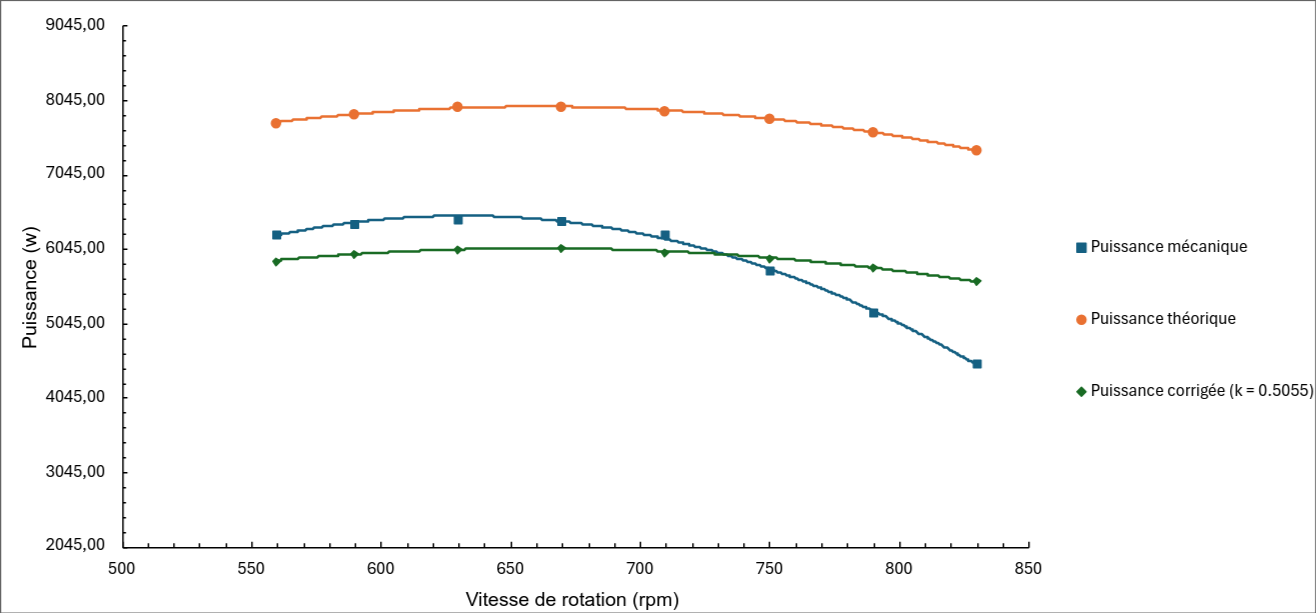
\includegraphics[width=\linewidth]{images/graphs/03_puissance_corrigee.png}
			\caption{Courbes de puissance en fonction de la vitesse : théorique et expérimentale.}
    			\label{fig:Graph13}
		\end{figure}
		\begin{figure}[H]
    			\centering
			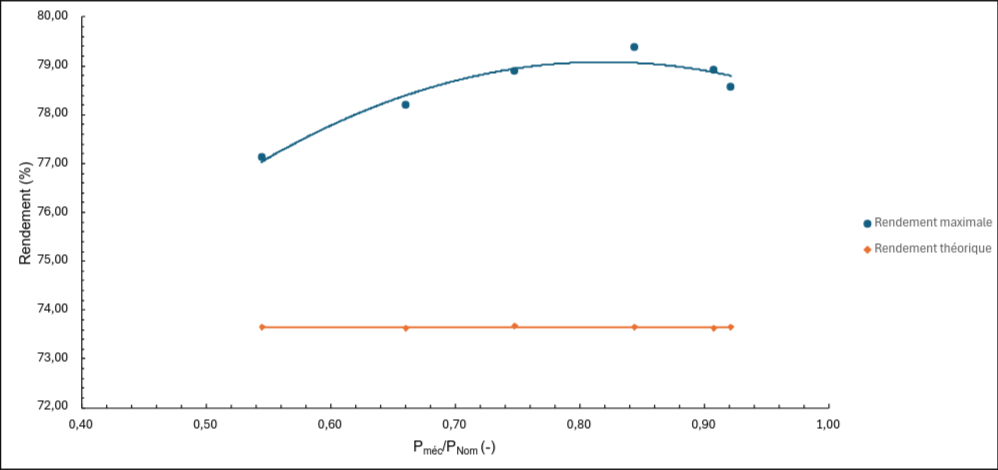
\includegraphics[width=\linewidth]{images/graphs/04_rendements_puissance_normalisee.png}
			\caption{Courbe du rendement maximal en fonction du pourcentage de la charge maximale
de la turbine.}
    			\label{fig:Graph14}
		\end{figure}
		\begin{table}[H]
    			\centering
    			\caption{Comparaison de la vitesse à la sortie du pointeau et en périphérie des auges au point de rendement maximal}
    \label{tab:Tab11}
    \begin{tabular}{|c|c|c|c|c|}
        \hline
	x [mm] & U [m/s] & $\frac{C_1}{2}$ & N [rpm] & Écart relatif entre U et $\frac{C_{1}}{2}$ [\%] \\
        \hline
	8 & 12.56  & 13.07 & 629.84 & 3.83 \\
        \hline
	10 & 12.58  & 13.14 & 630.48 & 4.30 \\
        \hline
	13 & 12.59  & 13.10 & 631.05 & 3.89 \\
        \hline
	16 & 12.55  & 13.00 & 629.22 & 3.45 \\
        \hline
	20 & 12.55  & 13.11 & 629.08 & 4.28 \\
        \hline
	23 & 12.57  & 13.05 & 630.29 & 3.62 \\
        \hline
    \end{tabular}
\end{table}		
		
\subsection{Étude sur le rendement et le rapport de vitesse de jet pour la turbine Pelton}
\begin{table}[H]
    \centering
    \caption{Valeurs nécessaires pour obtenir la vitesse de jet mesurée et vérification de $U = \frac{C_1}{2}$ au point de rendement maximal pour chaque ouverture du pointeau (données de 2019) }
    \label{tab:Tab14}
    \resizebox{\textwidth}{!}{
    \begin{tabular}{|c|c|c|c|c|c|c|c|c|c|c|c|c|c|}
        \hline
        x [mm] & N à $\eta_{\max}$ [rpm] & $\eta_{\max}$ [\%] & $P_{\text{méc}}$ [W] & $\frac{P_{\text{méc}}}{P_{\text{Nom}}}$ & $\eta_{\text{th}}$ au même point [\%] & Q [m$^3$/s] & H [m] & $C_1$ [m/s] & U [m/s] & $\frac{C_1}{2}$ [m/s] & $\frac{U}{C_1/2}$ & $\frac{C_1}{U}$ & Écart relatif entre U et $\frac{C_1}{2}$ [\%] \\
        \hline
        8  & 629.84 & 78.57 & 6452.43 & 0.92 & 73.64 & 0.02412 & 34.79 & 26.13 & 12.56 & 13.07 & 0.96 & 2.08 & 3.83 \\
        \hline
        10 & 630.48 & 78.91 & 6354.06 & 0.91 & 73.61 & 0.02337 & 35.20 & 26.29 & 12.58 & 13.14 & 0.96 & 2.09 & 4.30 \\
        \hline
        13 & 631.05 & 79.38 & 5908.63 & 0.84 & 73.64 & 0.02175 & 34.96 & 26.20 & 12.59 & 13.10 & 0.96 & 2.08 & 3.89 \\
        \hline
        16 & 629.22 & 78.88 & 5239.73 & 0.75 & 73.66 & 0.01970 & 34.45 & 26.00 & 12.55 & 13.00 & 0.97 & 2.07 & 3.45 \\
        \hline
        20 & 629.08 & 78.19 & 4628.89 & 0.66 & 73.62 & 0.01727 & 35.03 & 26.22 & 12.55 & 13.11 & 0.96 & 2.09 & 4.28 \\
        \hline
        23 & 630.29 & 77.11 & 3814.85 & 0.54 & 73.65 & 0.01457 & 34.69 & 26.09 & 12.57 & 13.05 & 0.96 & 2.08 & 3.62 \\
        \hline
    \end{tabular}
    }
\end{table}
